\documentclass[10pt,twocolumn]{IEEEtran11}

\usepackage{times}
\usepackage{epsfig}
\usepackage[T1]{fontenc}
\usepackage{graphicx}
\usepackage{subfigure}
\def\BibTeX{{\rm B\kern-.05em{\sc i\kern-.025em b}\kern-.08em
    T\kern-.1667em\lower.7ex\hbox{E}\kern-.125emX}}

\oddsidemargin -15pt
\evensidemargin -15pt
\leftmargin 0 pt
\topmargin -30pt
\textwidth = 6.9 in
\textheight = 9.0 in

\newcommand{\itembase}{\setlength{\itemsep}{0pt}}
\newcommand{\eg}{{\it e.g., }}
\newcommand{\ie}{{\it i.e., }}
\graphicspath{{FIG/}}

\begin{document}

\bibliographystyle{IEEE}

\title{\Large \bf A Comparison of Distributed Data Processing Systems}
\author{
Vincent M Chen\\
Information and Computer science Department\\
University of Oregon\\
{\em applekey@cs.uoregon.edu}
}
\maketitle

\section{Introduction}
The explosion of data in the past decade has lead to many questions in finding the most efficient method in order to analyze the data being generated. Best put by Google's CEO, Eric Schmidt, "There were 5 exabytes of information created by the entire world between the dawn of civilization and 2003. Now that same amount is created every two days.", more percisely, in 2003, 6.8 exabytes were being created every 2 days,\cite{gantz2010digital}.  With such a large volume of throughput, trivial tasks such as locating a users' account or finding all users within the same group can't be found in meaningful time with a single computers nor using sequential algorithms.
\par
In order to solve this problem, a very important insight is to notice that a large majority of the data being created is independent from each other, ex. different users on an on-line shopping platform where every shopper has their own independent profile, shopping cart and payment information.  Independence within the data means that parallel computation can be used, where instead of a single computer processing data sequentially, the job is divided into many sub tasks and processed in parallel.  This allows the computation of a large data set to be divided among the processing power of multiple computers.
\par
These parallel computation systems have existed since the 1980's, the most common of which are database systems. In the time since, many database systems have evolved into both parallel and distributed varieties.  As well, alternative computation frameworks introduced recently such as map reduce or Apache Spark have taken a  similarly approach to that used by databases, parallel computation.  The goal of this survey paper is to firstly introduce these different data query systems and their variants.  Secondly, discuss the common approaches all of them use to speed up computation and finally highlight unique aspects of each system.

\section{Basic Description of Functionality}

A data processing solution should satisfy the following functionality:
\begin{enumerate}	
	\item Guarantee high degree of fault tolerance.
	\item Compute a user defined query in a reasonable time.
\end{enumerate}

\subsection{Fault Tolerance}
Fault tolerance is the most important guarantee that a computation framework provides.  Without consistency, the data being returned from the query cannot be used for any meaningful analysis. Fault tolerance means recovery from failure from multiple sources

\begin{enumerate}
	\item Network fault, communication between compute nodes is unreliable and data is lost in between
	\item System fault, OS failure
	\item Hardware fault, compute computer hard disk fails
	\item User fault, user query has code that leaves query engine in a bad state
\end{enumerate}

In order for user defined queries to complete in a reasonable time, two levels of parallization can be applied.

\subsection{Parallel Computation}
The framework can process independent queries in parallel.  For example, searching for all students who owe more than 10,000 dollars in student loans
can be queried in parallel, each student can be treated independently.

\subsection{Distributed Computation}
The framework is able to distribute the data set across multiple compute machines.  Each machine might contain independent data, for example, one machine contains all students with first names starting A to J and another from K to Z.  Another case is multiple machines hold data that is related to one another.  For example in figure \ref{fig:distDataDependency}, machine A might hold all student's GPA and Awards and another machine holds the student's student loan amount.
If the query were to find all students that had more than 10,000 in student loans but also a 4.0 GPA in order to give them a financial award, then each query per student would need to look at the data in both compute machines.

\begin{figure}[h]
\centering
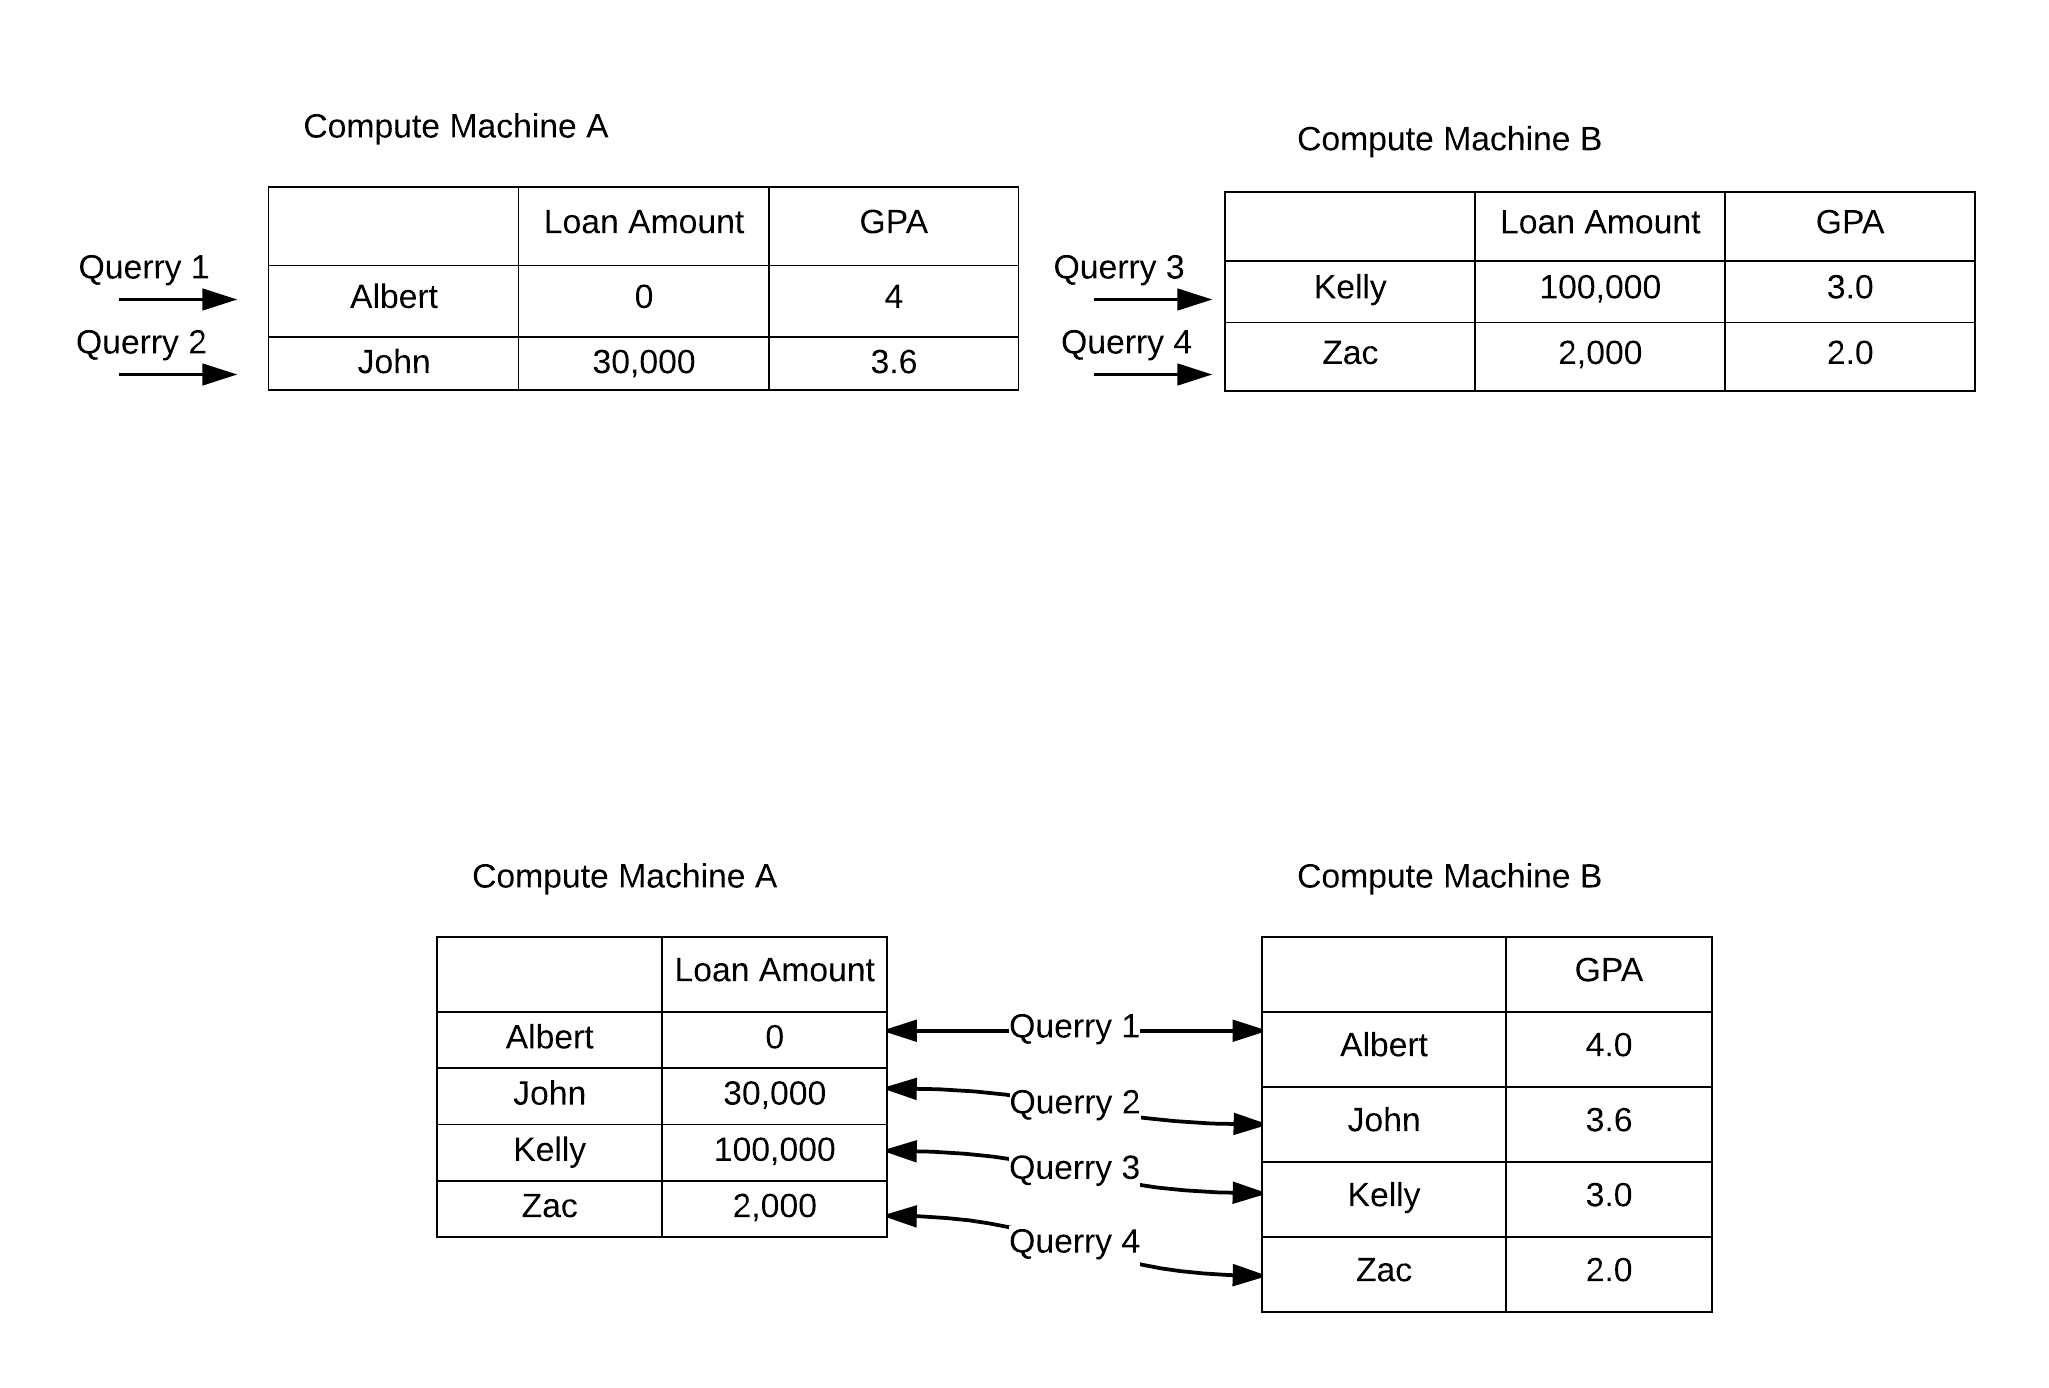
\includegraphics[scale=0.12]{images/parallelComputation.png}
\caption{Distributed Data Dependency}
\label{fig:distDataDependency}
\end{figure}


%-----------------------------------------------------Good ends here----------------------------------------------------------
\section{Databases Management Systems}

Databases management systems are systems that store data in tabular tables with set schemas.  DBMS systems use relational queries to perform CRUD 
(Create, read, update and delete)operations on the stored data.  

\fix{write more here}

\subsection{Parallel DBMS}

Relational queries are idealy suited to run parallel since they
each operation declares independant operations on independant data sets \cite{dewitt1992parallel}.  By partiioning the data amoung mulitple proessors, a single querry can be carried out in parallel and the result merged into a final step.  In figure \ref{fig:disDBMS}, an independant scan (ex, look for key word) is applied and the results are sorted (binned by first letter) and then the result of each independant operation is merged into the final result.

\begin{figure}[h]
\centering
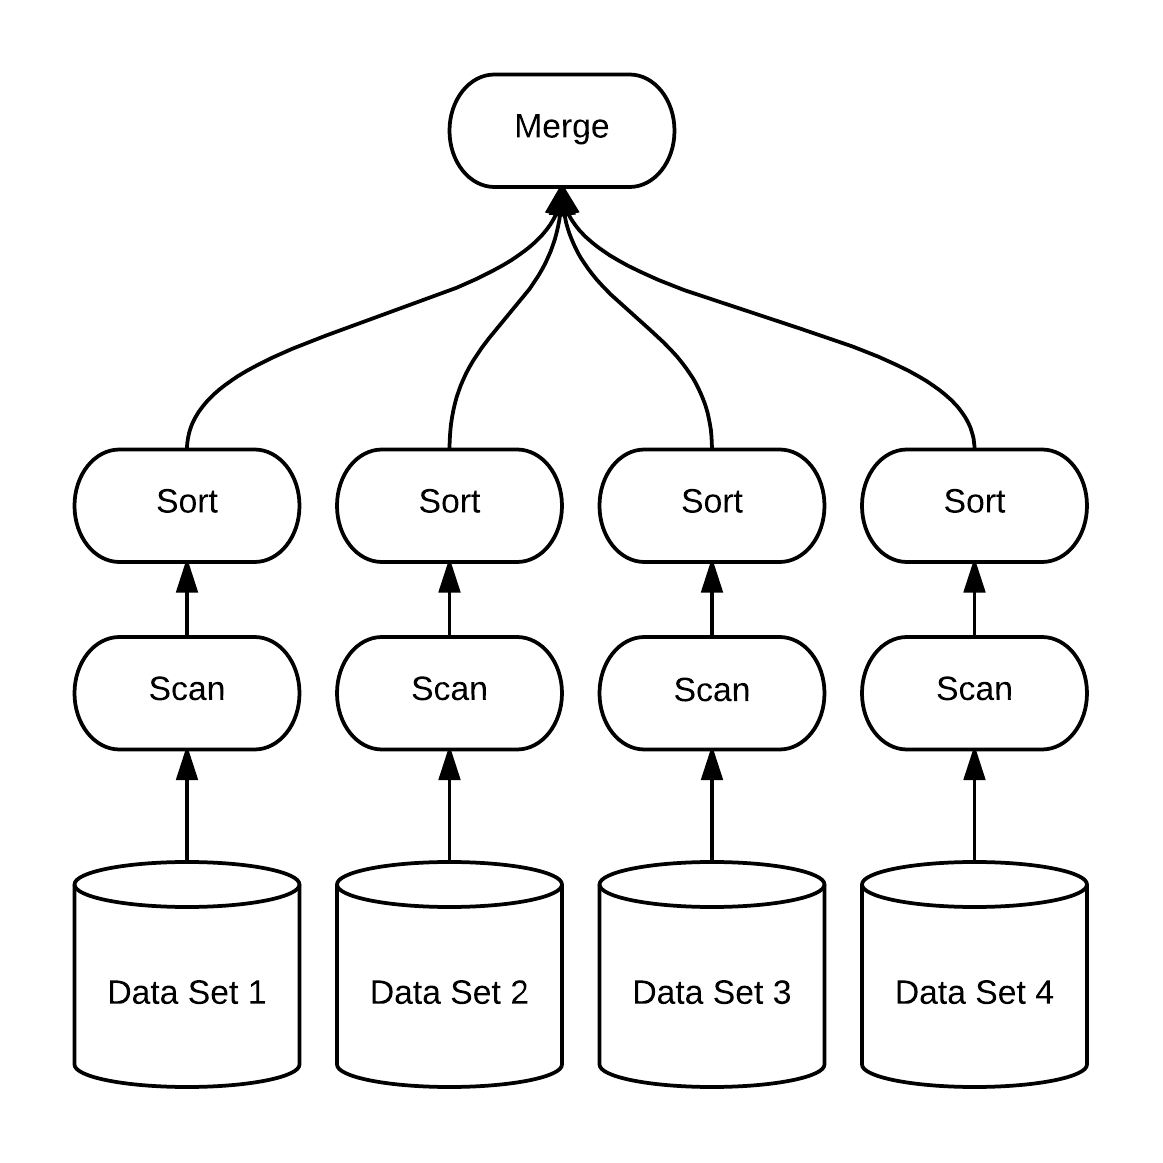
\includegraphics[scale=0.12]{images/parDBMS.png}
\caption{Distributed Data Dependency}
\label{fig:disDBMS}
\end{figure}

\subsection{Distributed DBMS}

Distributed DBMS systems require an additional layer of abstraction on top of Parallel DBMS.  Where as in parallel DBMS systems, all querries are run on the same machine sharing the same memory space.  Distributed DBMS systems need to consider the additonal factor of latency when access data that does not reside in the current compute machine.  Additionaly, distributed DBMS systems need to consider what impact does the memory laytout have in preventing easily addming more compute nodes.  

Generally speaking, there are three main types of memory 
archtectures for distributed DBMS systems, shared-nothing, shared-memory, shared-disk.

\begin{enumerate}
\item Shared-Memory: All compute machines share access to a global memory as well as disk storage.  
\item Shared-Disk: Each compute machines have their own memory, but share global disk.
\item Shared Nothing: Each compute machine has their own memory and disk. 
\end{enumerate}

\subsection{Fault Tolerance}


\section {Map Reduce}

Map Reduce is a general distributed computation framework introduced by Google in 2004 \cite{dean2001mapreduce}.  Map reduce is different from distributed DBMS systems in that much more general computations can be defined, not limited by the querry language of a rigit schema as is the case with DBMS systems.  Map Reduce, like DBMS systems have fault tolerance mechanisms but they operate differently than DBMS systems due to the archetcutral differences. 

\subsection{Mapper and Reducer}
Map reduce operates in two steps, the map step and then the reduce step.  Both steps are independant in that the reduce step will not start until all mappers have completed.
In the map stage, the data is partitioned equally among N mappers.  Input data arrives to the mapper as a list of (key, value) pairs, the mapper applies a user-defined map operation.
The map operation produces intermediate (key, value) pairs which are the results of the map operations.  
\par
The reducer is again a user defined operation that processes the intermediate values from the mapper grouped by key.  The reducer can produce zero or an aggregate of all values
that map to the same key.

Figure \ref{fig:mapReduce} gives an execution diagram.
\begin{figure}[h]
\centering
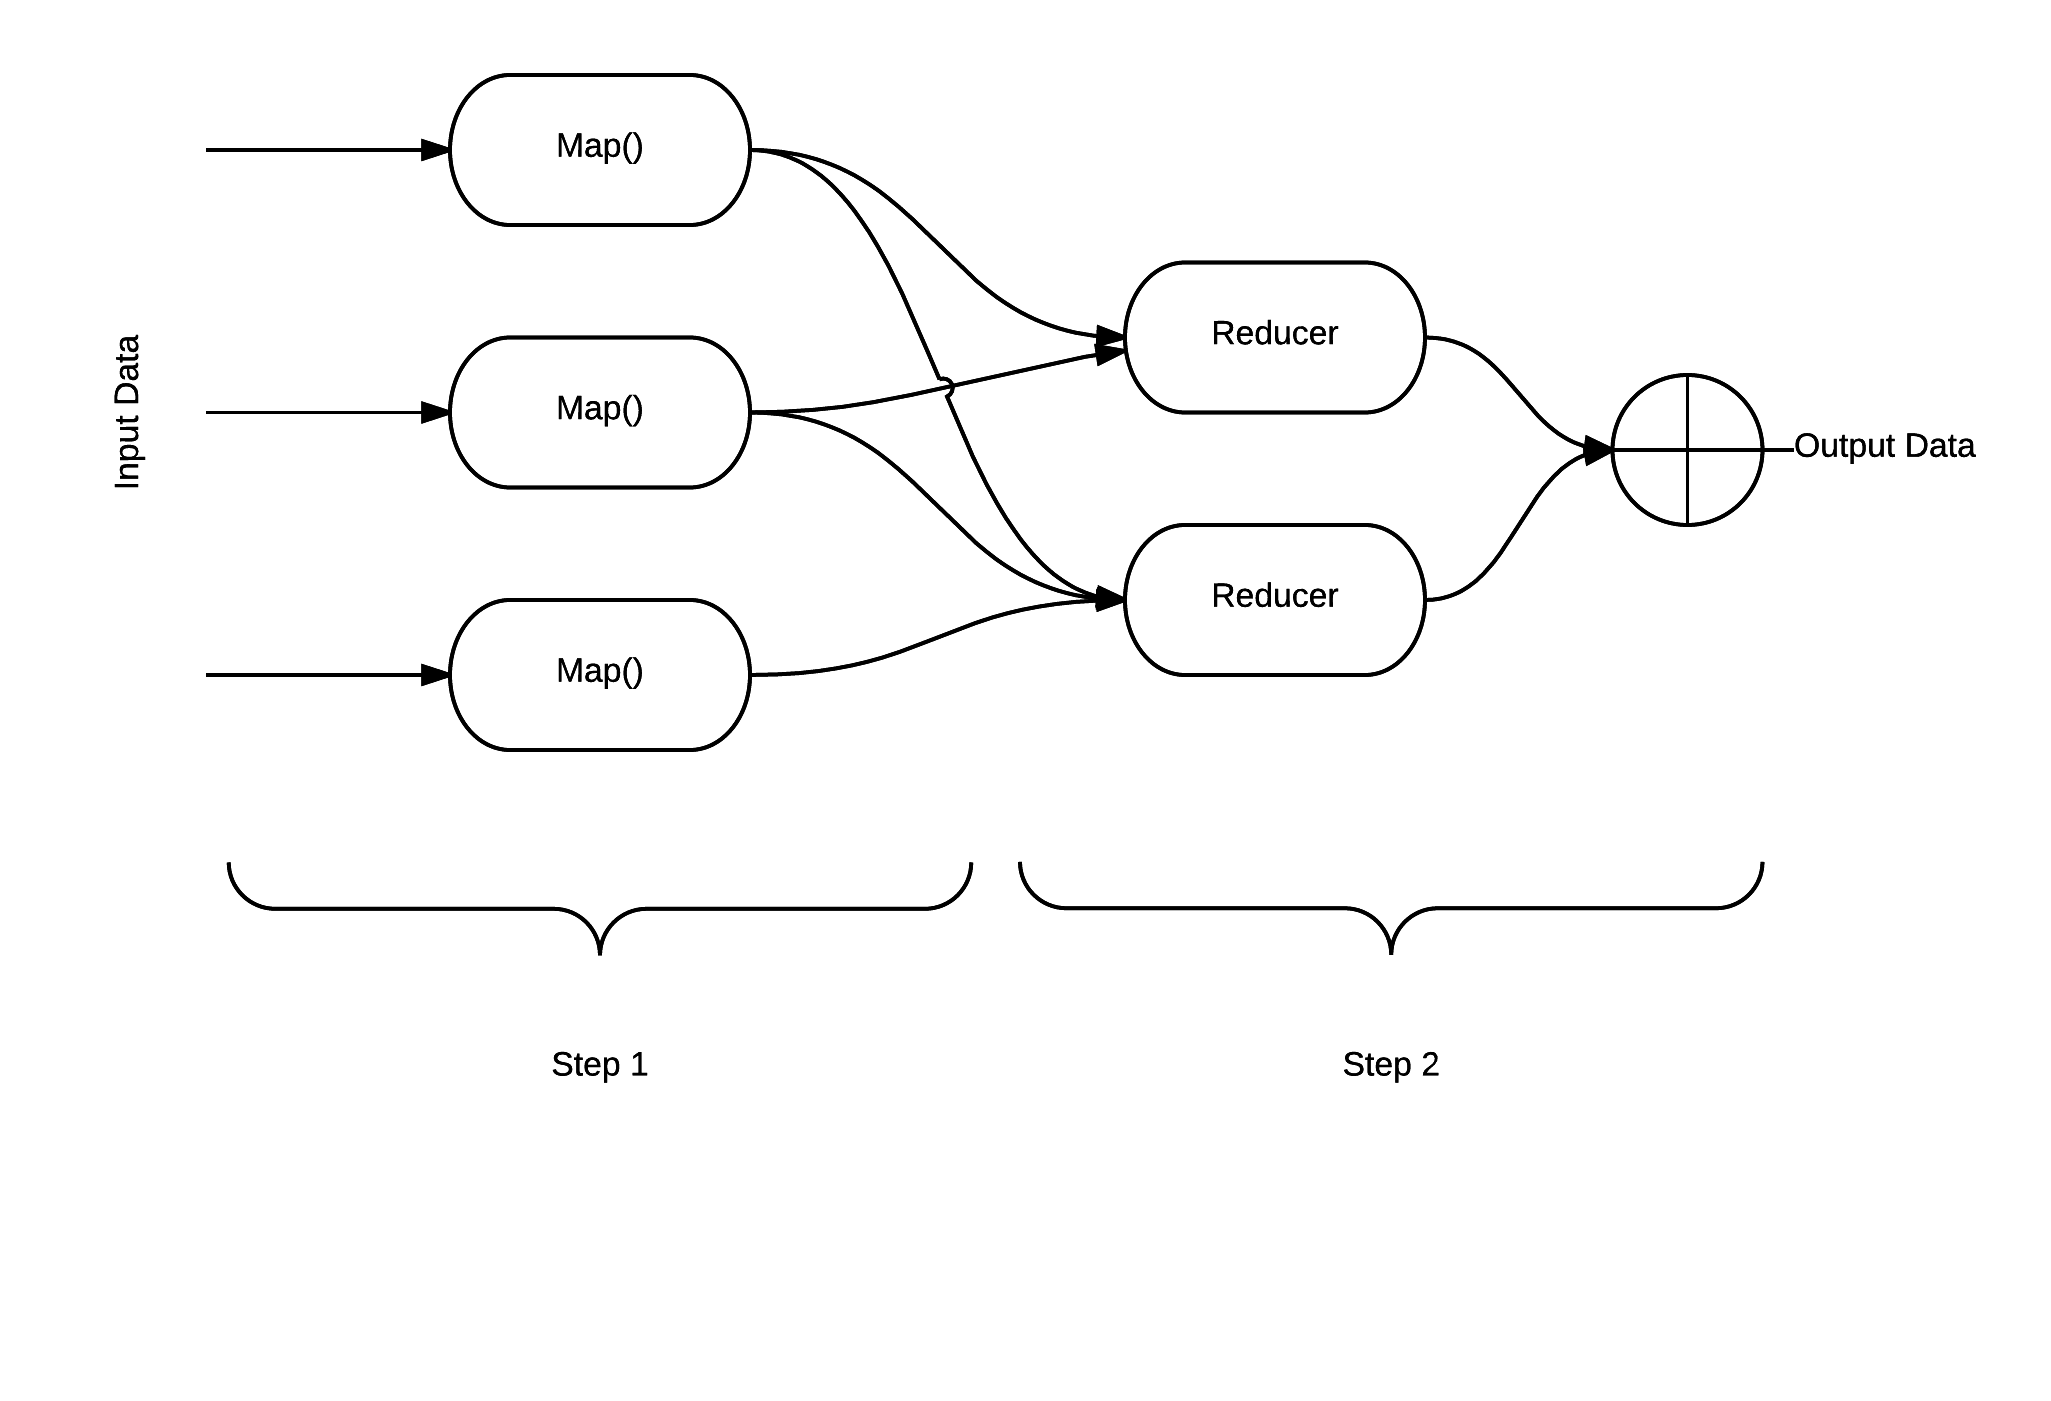
\includegraphics[scale=0.12]{images/mapReduce.png}
\caption{Map Reduce Program Execution}
\label{fig:mapReduce}
\end{figure}

\subsection{Hadoop}
There are two very popular frameworks that implmement the map reduce concept, these are the closed source Google Map Reduce and open source version Hadoop Map Reduce.  
This paper will focus on Hadoop instead of Google Map Reduce since the complete details of Google Map Reduce and relatively unknown, however both frameworks function similarly.
Hadoop has 




\subsection{Fault Tolerance}





Analgous to parallel DBMS, the map and reduce step are very similar to a filter and reduce.




















The Map Reduce model follows two core steps, the map step and then the reduce step.  Initially, data is fed into the map step as key value pairs.  The map step itself is user-defined filter that applies the filter to each entry of the input key value pairs.  The reduce step then aggregates the results of the first filter step into key value pairs of the first.
\par
The Hadoop implementation of Map Reduce is built upon a Data storage layer called the Hadoop DFS.  HDFS is a block-structured file system that is managed by a master node.  When the user specifies the data set that the map reduce program will operate on, the underlying HDFS will partition the data into multiple homogeneous blocks, typically about 64 MB and triple duplicate the input data to guarantee fault tolerance.  Each data block is then assigned to a mapper and the processes begins.
\par
Within each local data set, after the map has completed a local sort is applied in-order to combine entries that share the same key, for example, {k1, v1,v2,v3,v4}.  This is done in order to minimize the amount of data that has to be transfer ed inter node. A combine step can be applied furrther, for example v1+v2+v3+v5.  This data is then stored to disk, there is a barrier, once all the data partitions have being processed for the first step can then the reduce step proceed.  
\par
Just like with the map phase, the intermediate data is stored into R partitions, where R is the number of reduce processors.
\subsection{Architecture}
The Hadoop Map Reduce Architecture consist of three major components, the client, the master node and the slave nodes.  The client intially contains the data that needs to be analyzed, this can be un-structured data ex, web pages, system logs, simulation results.  The master node has two roles, the first is partition the data from the client to the hdfs and the second is assigning map reduce tasks to work on these data partitions.
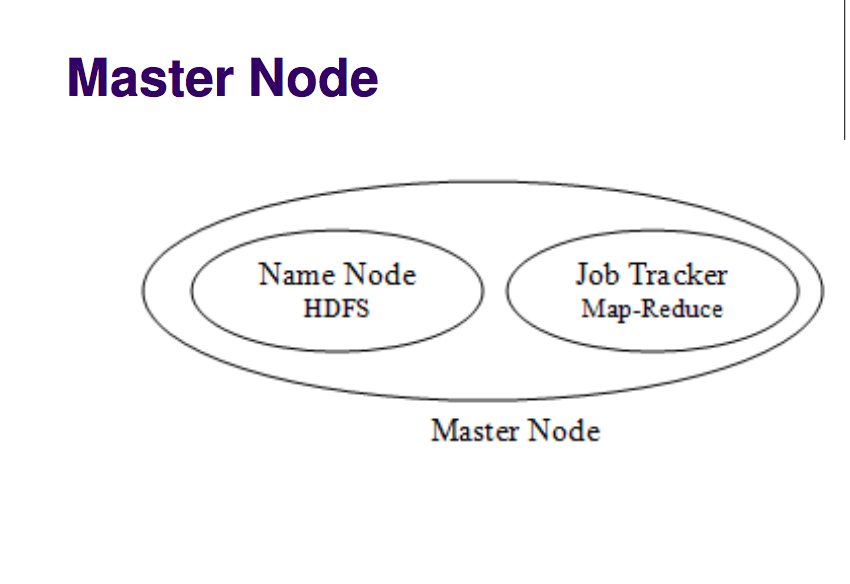
\includegraphics[width=6cm, height=6cm]{masterNode.png}
Within the master node, the Name Node helps in coordinating the hdfs and the job tracker helps in coordinating parallel execution of map reduce.
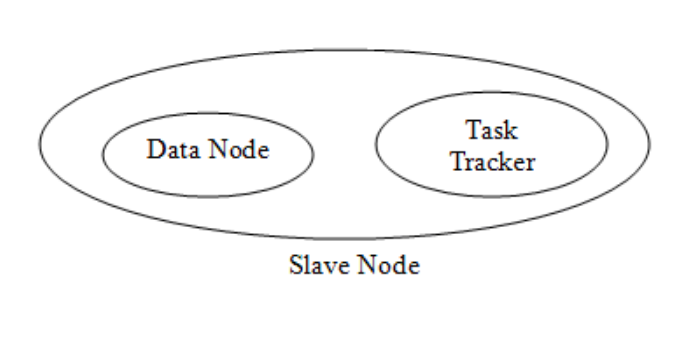
\includegraphics[width=6cm, height=6cm]{slaveNode.png}
The slave node communicate and recieve instructions from the master node and performs the map/reduce  tasks.
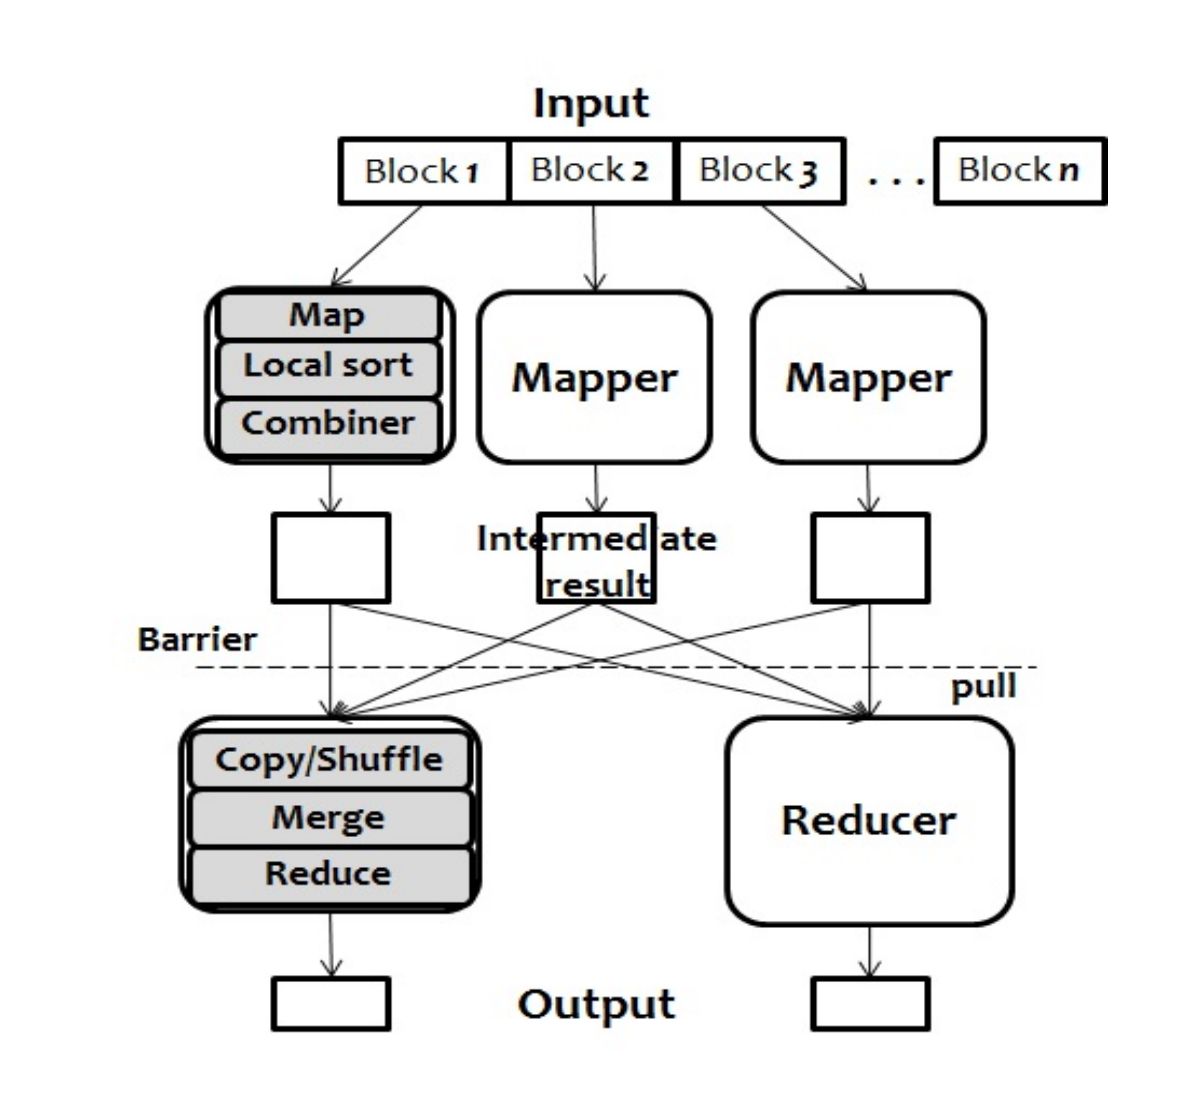
\includegraphics[width=6cm, height=6cm]{mapreduce.png}










Parallelism between DBMS systems can be roughly generalized into three types: shared- memory, shared-disk, and shared-nothing.




Shared-Nothing

A consensus on parallel and distributed database system architecture has emerged. This
architecture is based on a shared-nothing hardware design [STON86] in which processors
communicate with one another only by sending messages via an interconnection network. In
such systems, tuples of each relation in the database are partitioned (declustered) across disk
storage units
2 attached directly to each processor. Partitioning allows multiple processors to scan
large relations in parallel without needing any exotic I/O devices


shared-memory: All processors share direct access to a common global memory and to all
disks. The IBM/370, and Digital VAX, and Sequent Symmetry multi-processors typify this
design.

shared-disks: Each processor has a private memory but has direct access to all disks. The IBM
Sysplex and original Digital VAXcluster typify this design.



onsensus on parallel and distributed database system architecture has emerged. This
architecture is based on a shared-nothing hardware design [STON86] in which processors
communicate with one another only by sending messages via an interconnection network. In
such systems, tuples of each relation in the database are partitioned (declustered) across disk
storage units
2 attached directly to each processor. Partitioning allows multiple processors to scan
large relations in parallel without needing any exotic I/O devices. Such architectures were
pioneered by Teradata in the late seventies and by several research projects. This design is now
used by Teradata, Tandem, Oracle-nCUBE, and several other products currently underf


The main advantage of shared-nothing multi-processors is that they can be scaled up to
hundreds and probably thousands of processors that do not interfere with one another. Teradata,
Tandem, and Intel have each shipped systems with more than 200 processors. Intel is
implementing a 2000 node Hypercube. The largest shared-memory multi-processors currently
available are limited to about 32 processors.

\subsection{Factors that affect parallism}

The SQL data model was originally proposed to improve programmer productivity by
offering a non-procedural database language. Data independence was and additional benefit;
since the programs do not specify how the query is to be executed, SQL programs continue to
operate as the logical and physical database schema evolves.
Parallelism is an unanticipated benefit of the relational model. Since relational queries
are really just relational operators applied to very large collections of data, they offer many
opportunities for parallelism. Since the queries are presented in a non-procedural language, they
offer considerable latitude in executing the queries.
Relational queries can be executed as a dataflow graph. As mentioned in the
introduction, these graphs can use both pipelined parallelism and partitioned parallelism. If one
13
operator sends its output to another, the two operators can execute in parallel giving potential
speedup of two

The benefits of pipeline parallelism are limited because of three factors: (1) Relational
pipelines are rarely very long - a chain of length ten is unusual. (2) Some relational operators do
not emit their first output until they have consumed all their inputs. Aggregate and sort operators
have this property. One cannot pipeline these operators. (3) Often, the execution cost of one
operator is much greater than the others (this is an example of skew). In such cases, the speedup
obtained by pipelining will be very limited

\subsection{Data Partitioning}

Partitioning a relation involves distributing its tuples over several disks. Data partitioning
has its origins in centralized systems that had to partition files, either because the file was too big
for one disk, or because the file access rate could not be supported by a single disk. Distributed
databases use data partitioning when they place relation fragments at different network sites
[RIES78]. Data partitioning allows parallel database systems to exploit the I/O bandwidth of
multiple disks by reading and writing them in parallel. This approach provides I/O bandwidth
superior to RAID-style systems without needing any specialized hardware [SALE84, PATT88].
The simplest partitioning strategy distributes tuples among the fragments in a roundrobin
fashion. This is the partitioned version of the classic entry-sequence file. Round robin
partitioning is excellent if all applications want to access the relation by sequentially scanning all
of it on each query. The problem with round-robin partitioning is that applications frequently
want to associatively access tuples, meaning that the application wants to find all the tuples
having a particular attribute value. The SQL query looking for the Smith's in the phone book is
an example of an associative search.


Hash partitioning is ideally suited for applications that want only sequential and
associative access to the data. Tuples are place by applying a hashing function to the key
attribute of each tuple. The function specifies the placement of the tuple on a particular disk.
Associative access to the tuples with a specific attribute value can be directed to a single disk,
avoiding the overhead of starting queries on multiple disks. Hash partitioning mechanisms are
provided by Arbre, Bubba, Gamma, and Teradata.
Database systems pay considerable attention to clustering related data together in physical
storage. If a set of tuples are routinely accessed together, the database system attempts to store
them on the same physical page. For example, if the Smith's of the phone book are routinely
accessed in alphabetical order, then they should be stored on pages in that order, these pages
should be clustered together on disk to allow sequential prefetching and other optimizations.
Clustering is very application specific. For example, tuples describing nearby streets should be
clustered together in geographic databases, tuples describing the line items of an invoice should
be clustered with the invoice tuple in an inventory control application.
Hashing tends to randomize data rather than cluster it. Range partitioning clusters tuples
with similar attributes together in the same partition. It is good for sequential and associative
access, and is also good for clustering data. Figure 5 shows range partitioning based on
lexicographic order, but any clustering algorithm is possible. The B-tree is the most common
clustering algorithm. Range partitioning derives its name from the typical SQL range queries
such as
latitude BETWEEN 37
o AND 39
o
Arbre, Bubba, Gamma, Oracle, and Tandem provide range partitioning
The problem with range partitioning is that it risks datta skew, where all the data is place
in one partition, and execution skew in which all the execution occurs in one partition. Hashing
and round-robin are less susceptible to these skew problems. Range partitioning can minimize
skew by picking non-uniformly-distributed partitioning criteria. Bubba uses this concept by
considering the access frequency (heat) of each tuple when creating partitions a relation; the goal
being to balance the frequency with which each partition is accessed (its temperature) rather than
the actual number of tuples on each disk (its volume) [COPE88].


\subsection{parallism within nodes}
merge operator happens in different steps, data partitioning
Figure 7: Merging the inputs and partitioning the output of an operator. ***** jebus this is the same fucken thing as map/reduce


***********joins are the shit *************************


\section{Flexibility}
 
\section{Scalability}

\section{Efficiency}

\section{Fault tolerance}
































\subsection{Hadoop}
RAFTS:

    Hadoop has x mechanisms to handle failure for different granularity from failing nodes to failing map/reduce jobs.
The simplest mechanism is to reschedule the work from the failed node to another.  However, this scheme is correct only when operations are impotent.  
\par
The alternative is to checkpoint an ongoing computation, these checkpoints can be used to rollback failed states as well provide a intermediate stage to restart from instead of having to restart the whole computation.  There are three main challenges with this scheme.
(1) Checkpoints need a dependable and fault tolerant storage solution.  This extra layer adds complexity as well as decreases performance
(2) The stable storage solution will need to be able to handle the bandwidth from checkpoints for workers that it services.
(3) Recovering from failed tasks needs a dependane way to search for the correct checkpoint from stable storage and
send it back to a worker.  This taxes both IO as well as bandwidth.
\par
Previous implmentations of such systems that have attempted to address all three issues has significally decreased thhe perfomance of map/reduces [5], [6] http://ieeexplore.ieee.org/stamp/stamp.jsp?tp=&arnumber=5767877

\subsubsection{Failures}
Map reduce failures can be categorized into three types, master failures, worker failures and task failures.

- Task failures
task failures can occur from

bad data:

contention:
    for example there is a shared resouce that all nodes are trying to access, such as a local file system

medial corruption:
    for example disk corruption
    
bugs:
    there is a bug in the user-defined mapper/reducer
    

- Worker failures

These failures include hardware failures, these can be caused by physical damange of hardware such as overheating or wear and tear, very common with large data centers. When the master does not recieve an ping from a worker during a set amount of time, the master node will reschedule the mapper/reducer.

- master fialure:
master failure is the most simple to deal with, often the master node is replciated across multiple instance such upon failure, a backup instance is elected as the new master.


- Why failures are important

Based on the Facebook
application that loads 10 TB of compressed data per day [8],
assume that the size of relation R is 100 GB and that the size
of relation UV is 10 TB. Suppose that we want to analyze these
datasets using 100 workers, each being able to perform two
mappers concurrently. Using input splits of 256 MB — which
is a common configuration in practice — a single worker processes
on average (10.097 TB/100)/256 MB = 414 mappers.
As a worker runs two mappers concurrently, it requires 207
waves of mappers (with one wave we mean two concurrent
mappers). Based on the results for the join query presented
in [7], assume each mapper is processed in ∼17 seconds. Thus,
assuming perfect partitioning, 17 × 207 = 3, 519 seconds (≈1
hour) on average are required to perform the complete map
phase of our running example.
Since in MapReduce failures are the rule and not the
exception [1], let’s assume that each input split contains one
bad record in the middle, i.e. at offset 128MB. This is realistic
as MapReduce jobs often process large messy datasets and
thus can contain missing fields or incorrect formatting [9] —
e.g. the date format might be incorrect. As a result, any mapper
will fail just after ∼8.5 seconds of processing time. Recall that
MapReduce executes failing tasks twice before deciding to
skip a bad record [1]. Since each worker performs 207 waves
of mappers, the entire MapReduce job will be delayed by at
least 8.5 × 2 × 207 = 3, 519 seconds (≈1 hour) with a single
bad record per task. This is a 100% runtime overhead, which
clearly shows the need for more sophisticated algorithms that
allow for reducing delays caused by these failures.

\subsubsection{Checkpoints}

(1) Local Checkpointing (RAFT-LC). We exploit that MapReduce
persists intermediate results at several points in time
to checkpoint the computing progress done by mappers and
reducers. This enables MapReduce to resume tasks from last
checkpoints in case of task failure and hence to speed up
applications under these failures.
(2) Remote Checkpointing (RAFT-RC). We invert the way in
which reducers obtain their input from workers: we push
the intermediate results into all reducers as soon as results
are produced by mappers. This allows MapReduce to avoid
rescheduling completed mappers in case of worker failures.
However, notice that the intermediate results required by
local reducers will be lost in case of worker failure, because
such results are not pushed to remote workers. Therefore, we
replicate such intermediate results to remote workers.
(3) Query Metadata Checkpointing (RAFT-QMC). We identify
two problems when replicating intermediate results required
by local reducers, which may significantly decrease the performance
of applications. First, MapReduce jobs usually produce
large amounts of intermediate results. Second, RAFT-RC can
recover from only one worker failure. This is because a
failed reducer on any of the failed workers will require to
pull intermediate results produced by other failed workers.
Therefore, instead of replicating intermediate results required
by local reducers, we create and replicate a query metadata
checkpoint file. This file consists of the offset of all those
input key-value pairs that produce an intermediate result and
the identifier of the reducers that consume such results. As a
result, we are able to speed-up the re-computation of mappers
as well as to recover from more than one worker failure.

-------------results

-- input raft results here, some graphs

(1) Dealing with task failures (Section VII-E). In this series
of experiments, we focus on evaluating how well RAFT-LC
allows applications to recover from task failures.
(2) Dealing with worker failures (Section VII-F). In these
experiments we evaluate how well RAFT-RC and RAFT-QMC
allow applications to perform under worker failures.
(3) Putting everything together (Section VII-G). We focus on

-- end



Restarting whole operations can be both incorrect and inefficient.  If a node was near competition, the intermediate results can be used to resume a failed execution.  In order to take restart on intermediate results, te RAFT, Recovery Algorithm for Fast-Tracking in Map reduce was created by Quiane-Ruiz et al. [22].  Raft takes into account three types of check points
; local checkpoints (stores local mapper and reduce state), remote checkpoints, to store internemediate results of workers and querry meta dat acheckiingponts (to store the offset of input key-value pairs producing
the intermediate results).
    






\subsection{parallel dbms fault tolerance}

--- note that dbms systems rarely fail, thesei sbecause schema, more stable, built with stability in mind,
-- diffrent mind set

-- the week 9 lecture slides are pretty good

--- the book, checkpointing

- reliability protocols from Distributed and Parallel Database Systems


\section{optimizations}
\subsection{Hadoop}


Hadoop Map Reduce was designed first with simplicity and flexibility in mind, however in order to accommodate the two advantages mentioned, performance sometimes has to take a back seat. A fact that will be discussed in a further section, Hadoop runs significant slower than Parallel DBMS systems for a majority of category of general tasks. Compared with DBMS systems, Hadoop has 4 architectural disadvantages. These are:

\begin{itemize}
    \item Lack of high-level language 
        Coding map/reduce functors versus SQL queries has often being seen analogous to writing assembly.  Lacking a high level
        language increases the coding complexity, decreases probability as well as difficulty in understanding.  In addition, 
        high level query optimizations such as those with joins cannot be applied.
        \par
        The difference in Map/Reduce vs SQL programming approach was actually a well studied question in the 1970's.
        The database community discussed whether access programs should be written as
        \begin{itemize}
            \item By stating what you want - rather than presenting an algorithm for how to get it (relational view)
                    SQL querries are an example of this.
            \item By presenting an algorithm for data access (Codasyl view), Map Reduce is an example of this.
        \end{itemize}
        
        souce:http://db.cs.berkeley.edu/papers/pacific75-model.pdf
        
        It was determined that the advantage of the the relation view was
        \begin{itemize}
            \item Less source language statements to do a task
            \item Data Independence
            \item Sophistication of protection and integrity
        \end{itemize}
        
        Advantages of Procedural Languages
        \begin{itemize}
            \item Efficiency
        \end{itemize}
        
        
    \item Lack of data schema and index
        Map Reduce does not support schema's or indexing.  The lack of knowledge of the data model means that map reduce can only perform run-time optimisations.  Static optimisations such as *** can be performed by SQL because.  The simplest example where MR loses is data that is used between multiple MR jobs.  MR will need to load/save the data for each iterative MR stage, SQL engines would just leave the data loaded in memory. 
    
    \item Rigid data flow
        Map Reduce conceptually is very easy to understand.  There is a distinct map phase and another distinct reduce phase.  The reducers are only started when the mappers have all completed.  This rigid flow is far from optimal as it has being shown many times that multi-step reduction steps, a group that has finished is faster and more efficient. ** no paper reference here, should definitely find it.
    
    \item Poor run-time optimization
        In order to achieve both scalability as well as guarantee mapper/reduce fault tolerance, Map Reduce lacks efficient restart mechanisms.  When one MR instance fails, the whole instance is restarted.
        The Hadoop version of map reduce uses immutable strings as key/value pairs.  Each time any sort of transformation occurs, the immutable strings are destroyed and reallocated.
    
\end{itemize}

\subsection{Map Reduce Lacking}

souce https://homes.cs.washington.edu/~billhowe/mapreduce_a_major_step_backwards.html
4.  MapReduce is missing features

All of the following features are routinely provided by modern DBMSs, and all are missing from MapReduce:

Bulk loader -- to transform input data in files into a desired format and load it into a DBMS

Indexing -- as noted above

Updates -- to change the data in the data base

Transactions -- to support parallel update and recovery from failures during update

Integrity constraints -- to help keep garbage out of the data base

Referential integrity -- again, to help keep garbage out of the data base

Views -- so the schema can change without having to rewrite the application program


\subsection{Map Reduce Benchmarks}
source :http://database.cs.brown.edu/sigmod09/benchmarks-sigmod09.pdf

http://database.cs.brown.edu/papers/stonebraker-cacm2010.pdf
-> the second  one has a really good summary of the results

Map Reduce is on average 20 percent slower than DBMS in comparison for a variety of tasks.  Benchmarks in two category of tasks, data loading and analytical were run and run times between DBMS and Hadoop were compared.
\subsubsection{Data Loading}

The Data Loading benchmark was based on the original Map Reduce paper.  Both systems scanned through a data set of 100 byte records in order to look for a 3  character pattern.  The search pattern is only found in the last 90 bytes once every 10, 000 records.  The text data on each node is stored as plain text file.  The results for loading both the 535MB/node

// reword //reword
and 1TB/cluster data sets are shown in Figures 1 and 2, respectively.
For DBMS-X, we separate the times of the two loading phases,
which are shown as a stacked bar in the graphs: the bottom segment
represents the execution time of the parallel LOAD commands
and the top segment is the reorganization process. 
// reword //reword

--> Task Execution

Once data is loaded, a similar pattern search task in executed on each platform.  On the DBMS system, the query executed is SELECT * FROM Data WHERE field LIKE XYZ; Similarly, for Map Reduce, sub-string matching was performed on each value of all key-value pairs.  When the appropriate sub string is found, map/reduce will key/value onto the hdfs, there was no need for a reducer since no further aggregation is required.

In this test, Map Reduce performed far worse than Hadoop, lack of indexing and a set schema meant that execution times across all node sets and data sets were about 2x slower.

\subsubsection{Analytical}
Another set of more invoved computation were performed.  In this task, each task was given  600,000 unique HTML documents and links to other pages were generated
in a Zipfian distribution.

-> Data Loading


-> Selection/Aggregation/ Join/UDF task


\section{Map reduce optimizations}

source:http://www.cs.arizona.edu/~bkmoon/papers/sigmodrec11.pdf
In order to address the short comings of map reduce, the following application layer frameworks that sit on top of map reduce have being developed.

\subsection{High Level Languages}
Map Reduce's simplistic programming model means that there is a very gentle learning curve for new users to pick up.  But on the flip side, this means that more complex expressions  such as those for processing data from multiple data sets such as joins and N step data flows are missing.  What eventually happens is programmers have to stick together tightly cupleddata flows by hand and repleatly re-implenting standard functions in order to mesh with another stage.  This makes map reduce code difficult to understand, unportable and bug - prone.  

In order to address this short comming, Several high level languages have being developed as applications on top of hadoop.  Microsoft SCOPE[53], Apache Pig[22, 18], and Apache Hive[16, 17].  All three frameworks are designed with the three intentions in mind,
1) allow querry independannce from pogram logics, -> need to expand on this
2) allow reuse and modularity of querry
3) allow for automiatc querry opitmiation, such as those found for DBMS systems.

\subsection{Schemas}
Hadoop's version of Map Reduce suffer from inefficient repetitive serialize and serialization from key value pairs.  This occurs when one stage of a map reduce has  completed and the results and written to disk and re-read into the next stage.  Implementation becomes a large factor in performance when string values are seralized and deseralized repeattly.  The canonical version of Hadoop is written in Java, which supports immutatble strings, so any operations on key value paris requires allocating a new value and delete the old.  Each Map Reduce task is independent of other tasks, this is unlike DBMS systems where schema's and a declarative query language allow optimizing un-necessary loading and unloading of data between multiple task stages.
DBMS systems will initially load input data at the start of the very first stage, and index the data to allow for searching/ querying so that during runtime, the most efficient execution method is used.

Compression. We found that enabling
data compression in the DBMSs delivered
a significant performance gain.
The benchmark results show that using
compression in Vertica and DBMS-X on
these workloads improves performance
by a factor of two to four. On the other
hand, Hadoop often executed slower
when we used compression on its input
files; at most, compression improved
performance by 15%;

 We postulate that commercial
DBMSs use carefully tuned compression
algorithms to ensure that
the cost of decompressing tuples
does not offset the performance gains
from the reduced I/O cost of reading
compressed data. For example, we
have found that on modern processors
standard Unix implementations
of gzip and bzip are often too slow to
provide any benefit. 

\subsection{Data flow}

Map Reduce execution model is rigid in that there is a separation of a distinct map and reduce phase.  The reduce phase begins only when the all the mappers have completed and written their mapped data to the hdfs, remember that data is triple duplicated in the case of hadoop.  There are two performance bottlenecks with this simplistic approach.  Firstly, it has being show that partial map/ reduce steps are more efficient than a global one, this is called merge  map-reduce.  Secondly, and more importantly, Map Reduce does not support loop invariants,  For each iteration, if only one variable changes, all the mapped and reduce data has to be written to the FS, tripled duplicated and read back.
\par
Several frameowrks have attempted to solve both of these issues. HaLoop[66],
Twister[42], and Pregel[36] are application level systems that sit on top of hadoop
support loop programs in MapReduce.  

\subsubsection{Apache Spark}

\subsubsection{Haloop}

---reword rewrod

• New Programming Model and Architecture for Iterative Programs:
HaLoop handles loop control that would otherwise have
to be manually programmed. It offers a programming interface
to express iterative data analysis applications (Section 2).
• Loop-Aware Task Scheduling: HaLoop’s task scheduler enables
data reuse across iterations, by physically co-locating tasks that
process the same data in different iterations (Section 3).
• Caching for Loop-Invariant Data: HaLoop caches and indexes
data that are invariant across iterations in cluster nodes during
the first iteration of an application. Caching the invariant data
reduces the I/O cost for loading and shuffling them in subsequent
iterations (Section 4.1 and Section 4.3).
• Caching to Support Fixpoint Evaluation: HaLoop caches and
indexes a reducer’s local output. This avoids the need for a
dedicated map-reduce step for fixpoint or convergence checking
(Section 4.2).
• Experimental Study: We evaluated our system on iterative
programs that process both synthetic and real world datasets.
HaLoop outperforms Hadoop in all metrics; on average, HaLoop
reduces query runtimes by 1.85, and shuffles only 4% of the data
between mappers and reducers (Section 5).

\subsection{twister}

-- reword rewrod
Twister avoids instantiating workers repeatedly
during iterations. Previously instantiated workers
are reused for the next iteration with different inputs
in Twister. HaLoop is similar to Twister, and it also
allows to cache both each stage’s input and output to
save more I/Os during iterations



\subsection{Novelty}

source :
3. MapReduce is not novel

The MapReduce community seems to feel that they have discovered an entirely new paradigm for processing large data sets. In actuality, the techniques employed by MapReduce are more than 20 years old. The idea of partitioning a large data set into smaller partitions was first proposed in "Application of Hash to Data Base Machine and Its Architecture" [11] as the basis for a new type of join algorithm. In "Multiprocessor Hash-Based Join Algorithms," [7], Gerber demonstrated how Kitsuregawa's techniques could be extended to execute joins in parallel on a shared-nothing [8] cluster using a combination of partitioned tables, partitioned execution, and hash based splitting. DeWitt [2] showed how these techniques could be adopted to execute aggregates with and without group by clauses in parallel. DeWitt and Gray [6] described parallel database systems and how they process queries. Shatdal and Naughton [9] explored alternative strategies for executing aggregates in parallel.   

Teradata has been selling a commercial DBMS utilizing all of these techniques for more than 20 years; exactly the techniques that the MapReduce crowd claims to have invented.   

While MapReduce advocates will undoubtedly assert that being able to write MapReduce functions is what differentiates their software from a parallel SQL implementation, we would remind them that POSTGRES supported user-defined functions and user-defined aggregates in the mid 1980s. Essentially, all modern database systems have provided such functionality for quite a while, starting with the Illustra engine around 1995.  

\subsection{hadoop optimizations}

--











Existing architecture employs Schema-onWrite
(RDBMS) model
 Create Schema
 Transform data so as to fits it into this schema.
 Load data.
 Obtain required information.
 Efficient for compression, indexing,
partitioning but difficult to adapt to changes.

\section{Extra}
https://www.cs.uic.edu/~ajayk/c566/HadoopMap-Reduce.pdf










\bibliography{citations}


\end{document}
